% Le titre de la partie
\section{\trdpti}

%%%%%%%%%%%%%%%%%%%%%%%%%%%%%%%%%%%%%%%%%%%%%%%%
% Première diapo
%%%%%%%%%%%%%%%%%%%%%%%%%%%%%%%%%%%%%%%%%%%%%%%%

\begin{frame}
\frametitle{\trdpti}
\framesubtitle{}

    \centering {\huge \trdpti}

\end{frame}

%%%%%%%%%%%%%%%%%%%%%%%%%%%%%%%%%%%%%%%%%%%%%%%%
% Deuxième diapo
%%%%%%%%%%%%%%%%%%%%%%%%%%%%%%%%%%%%%%%%%%%%%%%%

\begin{frame}
    \frametitle{\trdpti}
    \framesubtitle{Parrallélisme: La carte graphique}
    
    \centering
    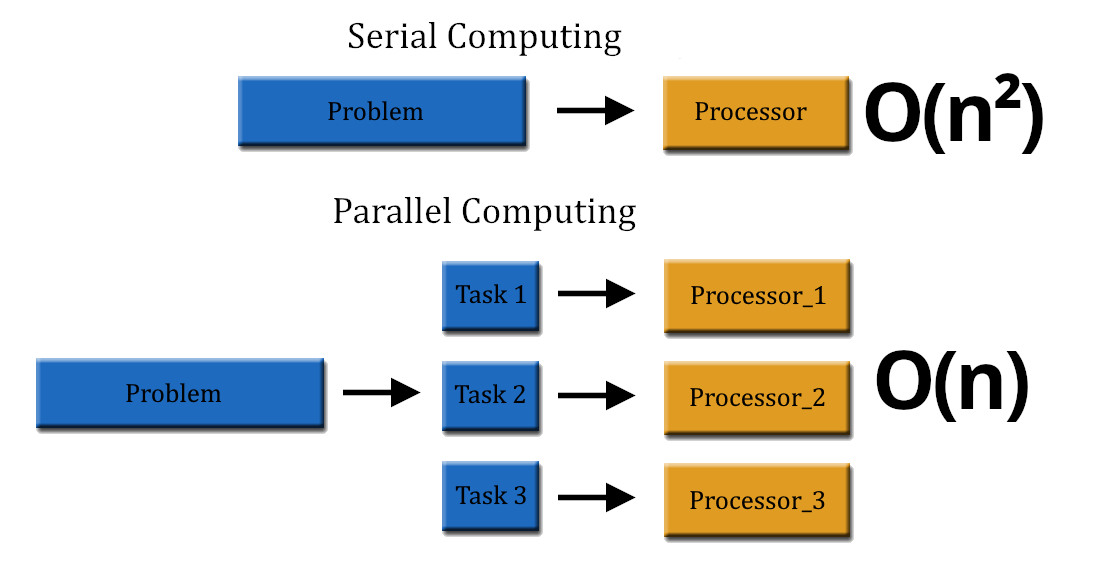
\includegraphics[width=1.0\linewidth]{figures/parallel_computing_vs_sequential_computing.png}
    
\end{frame}


%%%%%%%%%%%%%%%%%%%%%%%%%%%%%%%%%%%%%%%%%%%%%%%%
% Troisième diapo
%%%%%%%%%%%%%%%%%%%%%%%%%%%%%%%%%%%%%%%%%%%%%%%%

\begin{frame}
    \frametitle{\trdpti}
    \framesubtitle{Partitionnement de l'espace}
    
    \centering
    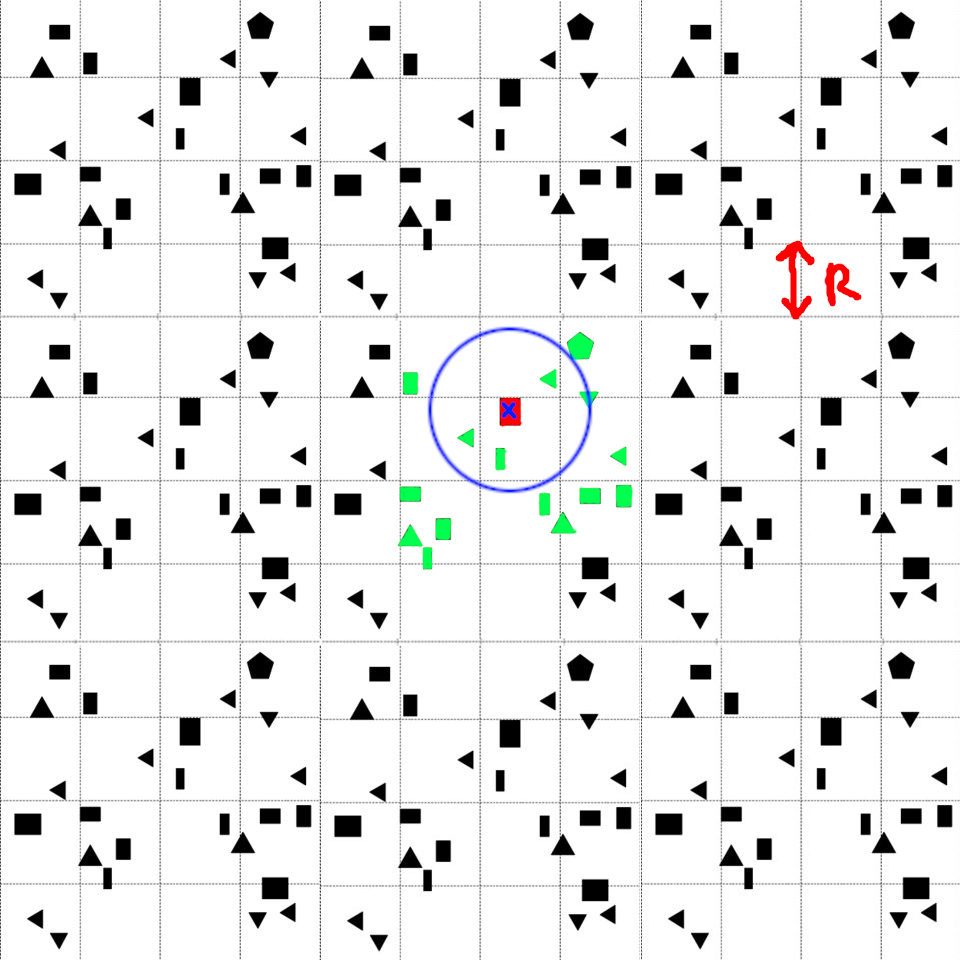
\includegraphics[width=0.75\linewidth]{figures/big_uniform_grid_partitionning.png}
    
\end{frame}


%%%%%%%%%%%%%%%%%%%%%%%%%%%%%%%%%%%%%%%%%%%%%%%%
% Quatrième diapo
%%%%%%%%%%%%%%%%%%%%%%%%%%%%%%%%%%%%%%%%%%%%%%%%

\begin{frame}
    \frametitle{\trdpti}
    \framesubtitle{Explication de l'algorithme de partitionnement}
    
    \onslide*<1-2>{ \centering {\huge
    [\textcolor{red}{0}, \textcolor{red}{1}, \textcolor{red}{2}, \textcolor{red}{3},
     \textcolor{red}{4}, \textcolor{red}{5}, \textcolor{red}{6},
    \textcolor{red}{7}, \textcolor{red}{8}, \textcolor{red}{9}]}}

    \onslide*<3>{ \centering {\huge
    [\textcolor{red}{0}, \textcolor{red}{1}, \textcolor{red}{2}, \textcolor{red}{3},
     \textcolor{red}{4}, \textcolor{red}{5}, \textcolor{red}{6},
    $\overset{\textcolor{red}{7}}{\textcolor{green}{2}}$, \textcolor{red}{8}, \textcolor{red}{9}]}}

    \onslide*<4>{ \centering {\huge
    [
    $\overset{\textcolor{red}{0}}{\textcolor{green}{9}}$,
    $\overset{\textcolor{red}{1}}{\textcolor{green}{0}}$,
    $\overset{\textcolor{red}{2}}{\textcolor{green}{6}}$,
    $\overset{\textcolor{red}{3}}{\textcolor{green}{7}}$,
    $\overset{\textcolor{red}{4}}{\textcolor{green}{1}}$,
    $\overset{\textcolor{red}{5}}{\textcolor{green}{1}}$,
    $\overset{\textcolor{red}{6}}{\textcolor{green}{4}}$,
    $\overset{\textcolor{red}{7}}{\textcolor{green}{2}}$,
    $\overset{\textcolor{red}{8}}{\textcolor{green}{2}}$,
    $\overset{\textcolor{red}{9}}{\textcolor{green}{2}}$
    ]}}

    \onslide*<5>{ \centering Liste spatiale: {\huge
    [
    $\overset{\textcolor{red}{1}}{\textcolor{green}{0}}$,
    $\overset{\textcolor{red}{4}}{\textcolor{green}{1}}$,
    $\overset{\textcolor{red}{5}}{\textcolor{green}{1}}$,
    $\overset{\textcolor{red}{7}}{\textcolor{green}{2}}$,
    $\overset{\textcolor{red}{8}}{\textcolor{green}{2}}$,
    $\overset{\textcolor{red}{9}}{\textcolor{green}{2}}$,
    $\overset{\textcolor{red}{6}}{\textcolor{green}{4}}$,
    $\overset{\textcolor{red}{2}}{\textcolor{green}{6}}$,
    $\overset{\textcolor{red}{3}}{\textcolor{green}{7}}$,
    $\overset{\textcolor{red}{0}}{\textcolor{green}{9}}$
    ]}

    \vspace{10px}

    Liste des départs: {\big [ $0$, $1$, $3$, $+\infty$, $6$, $+\infty$, $8$, $+\infty$, $9$]
    }}

    \onslide*<2-3>{
        \centering
        Indice: 7 \\
        Coordonnées de la case: $(4,1)$ \\
        Hachage des coordonnées: $4532$ \\
        Clé de la cellule: $4532 \mod 10 = 2$
    }

    \onslide*<1->{
        \centering
        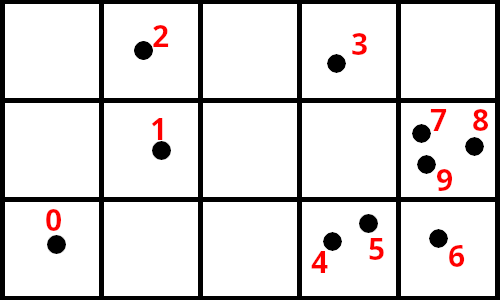
\includegraphics[width=0.5\linewidth]{figures/grid_partitionning_explanation_1.png}
    }
    
\end{frame}

%%%%%%%%%%%%%%%%%%%%%%%%%%%%%%%%%%%%%%%%%%%%%%%%
% Cinquième diapo
%%%%%%%%%%%%%%%%%%%%%%%%%%%%%%%%%%%%%%%%%%%%%%%%

\begin{frame}
    \frametitle{\trdpti}
    \framesubtitle{Tri bitonique}
    
    \centering
    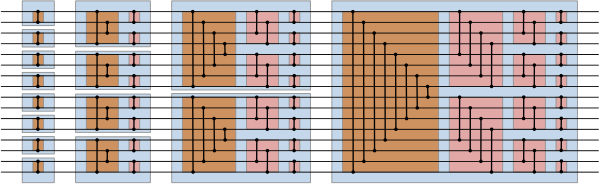
\includegraphics[width=1.0\linewidth]{figures/bitonic_sort.png}
    
\end{frame}
